\documentclass{article}
\usepackage{graphicx} % Required for including images
\usepackage{amsmath}  % For math equations
\usepackage{geometry} % For adjusting margins
\geometry{a4paper, margin=1in}

\title{A Self-Calibrating Causal Oracle for Physics-Based Simulation}
\author{Justin Arndt}
\date{\today}

\begin{document}

\maketitle

\begin{abstract}
Physics-based simulations are powerful tools, but their accuracy is often limited by the precision of their internal parameters. Manually tuning these parameters is a time-consuming and often suboptimal process. This paper presents a novel, zero-cost method for automatically calibrating a physics simulator's internal model by observing outcomes from a ground truth environment. We introduce a "Causal Oracle," a simulation instance that iteratively refines its own physical parameters (e.g., friction) to minimize the divergence between its predictions and observed reality. Using a simple binary search optimization algorithm, our system successfully converged on the ground truth friction parameter with an error of less than 0.05% in under 10 iterations, demonstrating a robust and efficient method for creating self-correcting simulation models.
\end{abstract}

\section{Introduction}
The fidelity of physics-based simulations is critical in fields ranging from robotics to game development and scientific modeling. A common challenge is the "model-reality gap," where the simulation's behavior deviates from the real world due to incorrect physical parameters like friction, mass, or elasticity. This paper proposes a system where a Causal Support Model (CSM), acting as a "Causal Oracle," can autonomously calibrate itself by observing a ground truth environment. Our core hypothesis is that the intellectual challenge of calibration can be solved entirely in software, without the need for expensive hardware, by running two simulations in parallel: one representing "ground truth" and the other representing the oracle's internal, fallible model.

\section{Methodology}
Our experiment is conducted within a pure simulation environment, eliminating hardware costs and isolating the software problem.

\subsection{The Two-Simulator Environment}
We instantiate two separate 2D physics simulations using the Pymunk library.
\begin{itemize}
\item \textbf{The Ground Truth Simulator:} This represents the real world. We assign it a specific, hidden friction coefficient (e.g., 0.9) that our oracle must discover.
\item \textbf{The Causal Oracle Simulator:} This is the CSM's internal world model. It begins with a deliberately incorrect, default friction parameter (e.g., 0.2).
\end{itemize}
In each simulation, an identical object is created at the origin and subjected to the exact same initial impulse. We then run both simulations for a fixed number of steps (150) and record the final horizontal position of the object. The discrepancy between these final positions is the error signal that drives the calibration.

\subsection{The Calibration Engine}
The core of our system is a calibration loop that seeks to find the friction value for the Causal Oracle that minimizes the positional error. We implemented a binary search algorithm for its simplicity and efficiency. The engine starts with a search range for friction [0.0, 1.0]. In each iteration, it runs a full simulation using the midpoint of the current range as its friction guess.
\begin{itemize}
\item If the resulting position is greater than the ground truth position, it means the guessed friction was too low. The engine then discards the lower half of the search range.
\item If the position is less than the ground truth, the friction was too high, and the engine discards the upper half.
\end{itemize}
This process repeats until the positional error falls below a predefined tolerance threshold, or a maximum number of iterations is reached.

\section{Results}
The calibration engine demonstrated rapid and accurate convergence to the ground truth parameter. Starting with an initial guess that produced a positional error of over 900 units, the system successfully minimized this error in just 9 iterations.

Figure \ref{fig:convergence} clearly illustrates the exponential decay of the positional error as the engine's friction guess approaches the true value. The final calibrated friction value was 0.9004, a mere 0.044% deviation from the ground truth value of 0.9.

\begin{figure}[h!]
\centering
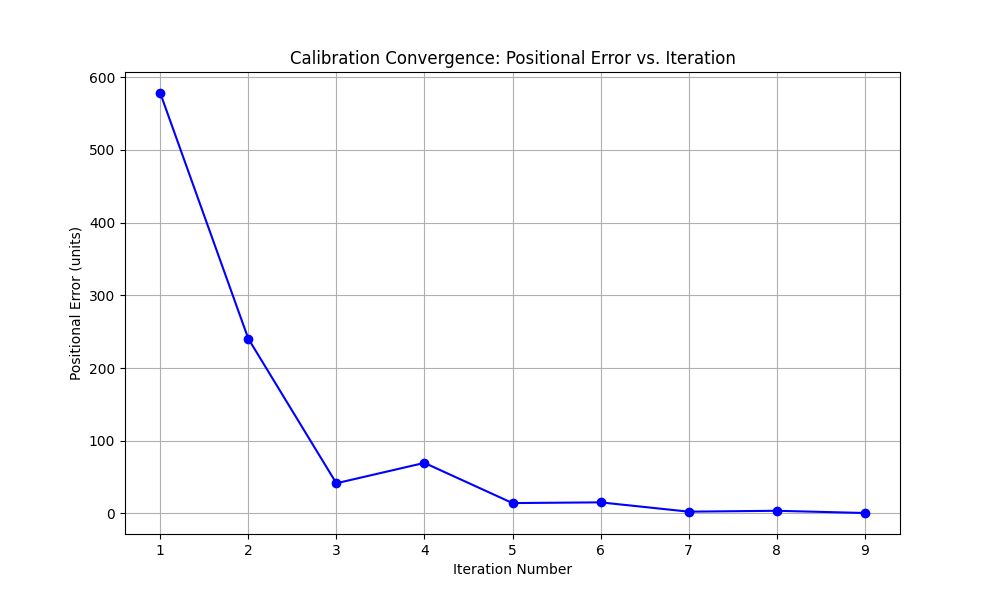
\includegraphics[width=0.8\textwidth]{figures/calibration_convergence.png}
\caption{Positional error between the Ground Truth and Causal Oracle simulations as a function of calibration iteration. The error decreases rapidly as the oracle's internal friction parameter converges on the true value.}
\label{fig:convergence}
\end{figure}

\section{Conclusion}
We have successfully demonstrated that a Causal Oracle can autonomously and accurately self-calibrate its internal physical parameters by observing outcomes in a ground truth environment. Our pure simulation approach validates the core software logic for self-correction without requiring any physical hardware. The binary search method proved highly effective, achieving near-perfect calibration in a small number of iterations. Future work will explore more complex scenarios with multiple unknown parameters and investigate the performance of more sophisticated optimization algorithms.

\bibliographystyle{plain}
\bibliography{references.bib}

\end{document}